\documentclass[norsk,a4paper,12pt]{article}
\usepackage[T1]{fontenc} %for å bruke æøå
\usepackage[utf8]{inputenc}
\usepackage{graphicx} %for å inkludere grafikk
\usepackage{verbatim} %for å inkludere filer med tegn LaTeX ikke liker
\usepackage{abstract}
\usepackage{hyperref}
\usepackage{gensymb}
\usepackage{booktabs}
\usepackage{multirow}
\usepackage{multicol}
\usepackage{siunitx}
\usepackage{fullpage}
\usepackage[font=scriptsize]{caption}
\bibliographystyle{plain}
\renewcommand{\thesection}{\Roman{section}} 
\usepackage[labelsep=period]{caption}
\renewcommand{\abstractnamefont}{\normalfont\normalsize\bfseries}
\renewcommand{\abstracttextfont}{\normalfont\small}
\setlength{\absleftindent}{0pt}
\setlength{\absrightindent}{0pt}
\makeatletter
\newcommand\footnoteref[1]{\protected@xdef\@thefnmark{\ref{#1}}\@footnotemark}
\makeatother
\usepackage{graphicx}
\usepackage{caption}
\usepackage{subcaption}
\usepackage{mhchem}
\newenvironment{Table}
   {\par\bigskip\noindent\minipage{\columnwidth}\centering}
   {\endminipage\par\bigskip}


\title{FYS4580 - OpenMC Project \\
\Large Final report}
\author{Julian Ersland Vevik}
\date{\today}
\begin{document}
\maketitle


\begin{abstract}
Two simulations have been made using the OpenMC Monte Carlo Code, where the properties of two different nuclear reactor configurations have been explored. First a pin-cell configuration for which a criticality of $k_{\infty} = 0.99552 \pm 0.00117$ was achieved using a moderator of $\ce{H_2O}$ with an added boron concentration of $670$ ppm. 
\\
Second, a thorium breeder reactor was simulated. Among others was the neutron and gamma flux found, in addition to calculating the fission yield products from a 15 day depletion chain simulation. This design was made critical using the same type of moderator as in the pin-cell, but with a boron concentration of $25633.0$ ppm. This gave a criticality of $k_{\text{eff}} = 0.99877 \pm 0.00129$. Furthermore, the possibility of commercial thorium reactors in Norway was discussed using the results from the simulations.
\end{abstract}



\setlength{\columnsep}{20pt}
\begin{multicols}{2}

\section{Introduction}
This project explores different aspects of nuclear reactor physics through simulations using the OpenMC Monte Carlo Code\cite{openmc}. First by looking at a basic pin-cell reactor, and then by extending this further to a full core thorium breeder reactor.

In the OpenMC code, a geometric setup must be constructed before one can start filling this with different materials. In the pin-cell a $\ce{UO_2}$ based fuel is used. The thorium breeder reactor uses a MOX fuel based on a $\ce{ThO_2}$-$\ce{PuO_2}$ blend. 

Investigations into how the criticality changes when altering the reactors in different ways are conducted, and an attempt is done to find a configuration for sustained critical and safe operation. 

The code for both reactor simulations can be found in a GitHub directory\cite{githubjulian}.
\section{Theory}
The criticality of a reactor is calculated using the five factor formula;
\begin{equation}
    k_{\text{eff}} = \eta f \varepsilon p P_{\text{NL}} ,
    \label{eq:keff}
\end{equation}
where $\eta$ is the reproduction factor, $f$ is the thermal utilization factor, $\varepsilon$ is the fast fission factor, $p$ is the resonance escape probability and $P_{\text{NL}}$ is the non-leakage probability.
\\
$\eta$ is defined as the ratio of the number of fast neutrons produced by thermal fission to the number of thermal neutrons absorbed in the fuel. $f$ describes how many of the thermal neutrons are absorbed in fuel material. $\varepsilon$ is the ratio of fast neutrons produced by fission in all energy ranges versus how many fast neutrons are produced in thermal fission. $p$ is the probability that the neutron will escape the resonance capture and become thermalized. The $P_{\text{NL}}$ term describes the probability that a neutron will leak out of the reactor.

In the infinite reactor case where the boundaries are reflective there is no leakage. The $P_{\text{NL}}$ factor would therefore equal 1, and in this case the infinite multiplication factor is found
\begin{equation}
    k_{\infty} = \eta f \varepsilon p .
    \label{eq:kinfinity}
\end{equation}




\section{The Pin-Cell}
A pin-cell, a heterogeneous infinite reactor lattice with reflecting boundary conditions, was modelled in OpenMC using a script called "PinCellNotebook.py" made by Sindre Hestnes Kaald\cite{sindrehk} as a basis. The script was altered to explore what happens to the criticality and other variables as different materials and radii etc. is changed. Throughout all of the simulations a number of 5000 particles and 100 batches(8 of them inactive) were used.

In this simplified pin-cell there is no leakage, and therefore the criticalities found are values for $k_{\infty}$ from Eq. \ref{eq:kinfinity}. When changing from light water, $\text{H}_{2}\text{O}$, to heavy water, $\text{D}_{2}\text{O}$, the expectation was that a higher criticality would be reached with the heavy water. The reason for this can be seen in Table \ref{tab:tab14nrp}, where the moderating ratio of heavy water is a lot higher than light water, even though it needs a few collisions more. Heavy water is much less likely to absorb neutrons since it already has one bound in the \ce{^{2}H}. 

\begin{Table}
\centering
\begin{tabular}{lrc}
\hline
\hline
Moderator & Collisions & $\xi \Sigma_s/\Sigma_a$ \\
\hline
\text{H}_{2}\text{O} & $16$ & $71$\\
\text{D}_{2}\text{O} & $29$ & $5670$\\
\hline
\hline
\end{tabular}
\captionof{table}{Number of collisions, on average, to moderate a neutron from 2 MeV to 1 eV. $\xi \Sigma_s/\Sigma_a$ is the moderating ratio which shows that $\text{D}_{2}\text{O}$ is less likely to absorb neutrons. Values taken from Nuclear Reactor Physics\cite{stacey} table 1.4.}
\label{tab:tab14nrp}
\end{Table}

However the results seemed to disagree with our initial thoughts, as can be seen in Table \ref{tab:kforh2oandd2o} where light water clearly has a higher criticality.

\begin{Table}
\centering
\begin{tabular}{lrc}
\hline
\hline
Moderator & $k_{\infty}$ \\
\hline
\text{H}_{2}\text{O} & $1.34108 \pm 0.00325$  \\
\text{D}_{2}\text{O} & $0.81386 \pm 0.00294$  \\
\hline
\hline
\end{tabular}
\captionof{table}{Criticalitites for $\text{H}_{2}\text{O}$ and $\text{D}_{2}\text{O}$ in the pin-cell with $\text{UO}_{2}$ fuel at $2.4\%$ enrichment. Pin size: fuel radius $r_f = 0.39218$, total radius with cladding $r_t = 0.45720$.}
\label{tab:kforh2oandd2o}
\end{Table}

The reason that the heavy water gave a lower criticality than light water is understood when looking at the geometry. With the radii that gave the results in Table \ref{tab:kforh2oandd2o}, the pin-cell was so large that the area where the moderator was outside the cladding was too small. Therefore the neutrons did not "spend enough time" in the moderator to collide enough times to be slowed down to the thermal region before escaping. This is an example that shows that even though heavy water has a higher moderating ratio it does need more collisions to moderate the neutrons, like seen in Table \ref{tab:tab14nrp}, and thus in this very particular case light water was better.

\begin{Table}
\centering
\begin{tabular}{lrc}
\hline
\hline
Moderator & $k_{\infty}$ \\
\hline
\text{H}_{2}\text{O} & $1.11023 \pm 0.00271$  \\
\text{D}_{2}\text{O} & $1.27710 \pm 0.00320$  \\
\hline
\hline
\end{tabular}
\captionof{table}{Criticalitites for $\text{H}_{2}\text{O}$ and $\text{D}_{2}\text{O}$ in the pin-cell with $\text{UO}_{2}$ fuel at $2.4\%$ enrichment. Pin size: fuel radius $r_f = 0.22$, total radius with cladding $r_t = 0.26$.}
\label{tab:kinflowerradius}
\end{Table}

Lowering the radius of the pin-cell meant that the amount of moderator covering it was larger, and therefore the heavy water proved a better moderator in this case, as seen in Table \ref{tab:kinflowerradius}. This is illustrated in Figure \ref{fig:pincell}, where it is evident how much more moderator is surrounding the pin-cell with the lower radius.

Increasing the criticality can also be done by increasing the enrichment of the Uranium in the fuel, i.e. increasing the percentage of \ce{^{235}U} compared to \ce{^{238}U}.

\multicolfloat{
    \begin{center}
	
\includegraphics[scale=0.033]{merge_from_ofoct.png}
	\captionof{figure}{The pin-cell with different radii. The left image shows the pin-cell with radius of fuel area $r_f = 0.39218$, and total radius with cladding $r_t = 0.45720$. The right shows the pin-cell with radius of fuel area $r_f = 0.22$, and total radius with cladding $r_t = 0.26$. Colors: $\text{UO}_2$ fuel is yellow, helium in gap is green, zirconium-alloy cladding is light brown and water(moderator) is light blue. }
	\label{fig:pincell}
	\end{center}
}


The energy distribution of the neutron flux for \ce{H_{2}O} and \ce{D_{2}O} can be seen in Figures \ref{fig:fluxh2o} and \ref{fig:fluxd2o} respectively. These distributions does not look like the prompt fission spectrum because the neutrons are moderated. Therefore there are peaks in the thermal neutron energy region as seen in the figures. There is also some evidence of the fact that light water needs fewer collisions to moderate the neutrons, in that there are more defined peaks and a lower flux in the areas between the fast and thermal neutron regions. In Fig. \ref{fig:fluxd2o} there is a more constant flux from the fast region all the way down to the thermal, where there is a peak. 

\multicolfloat{
    \begin{center}
	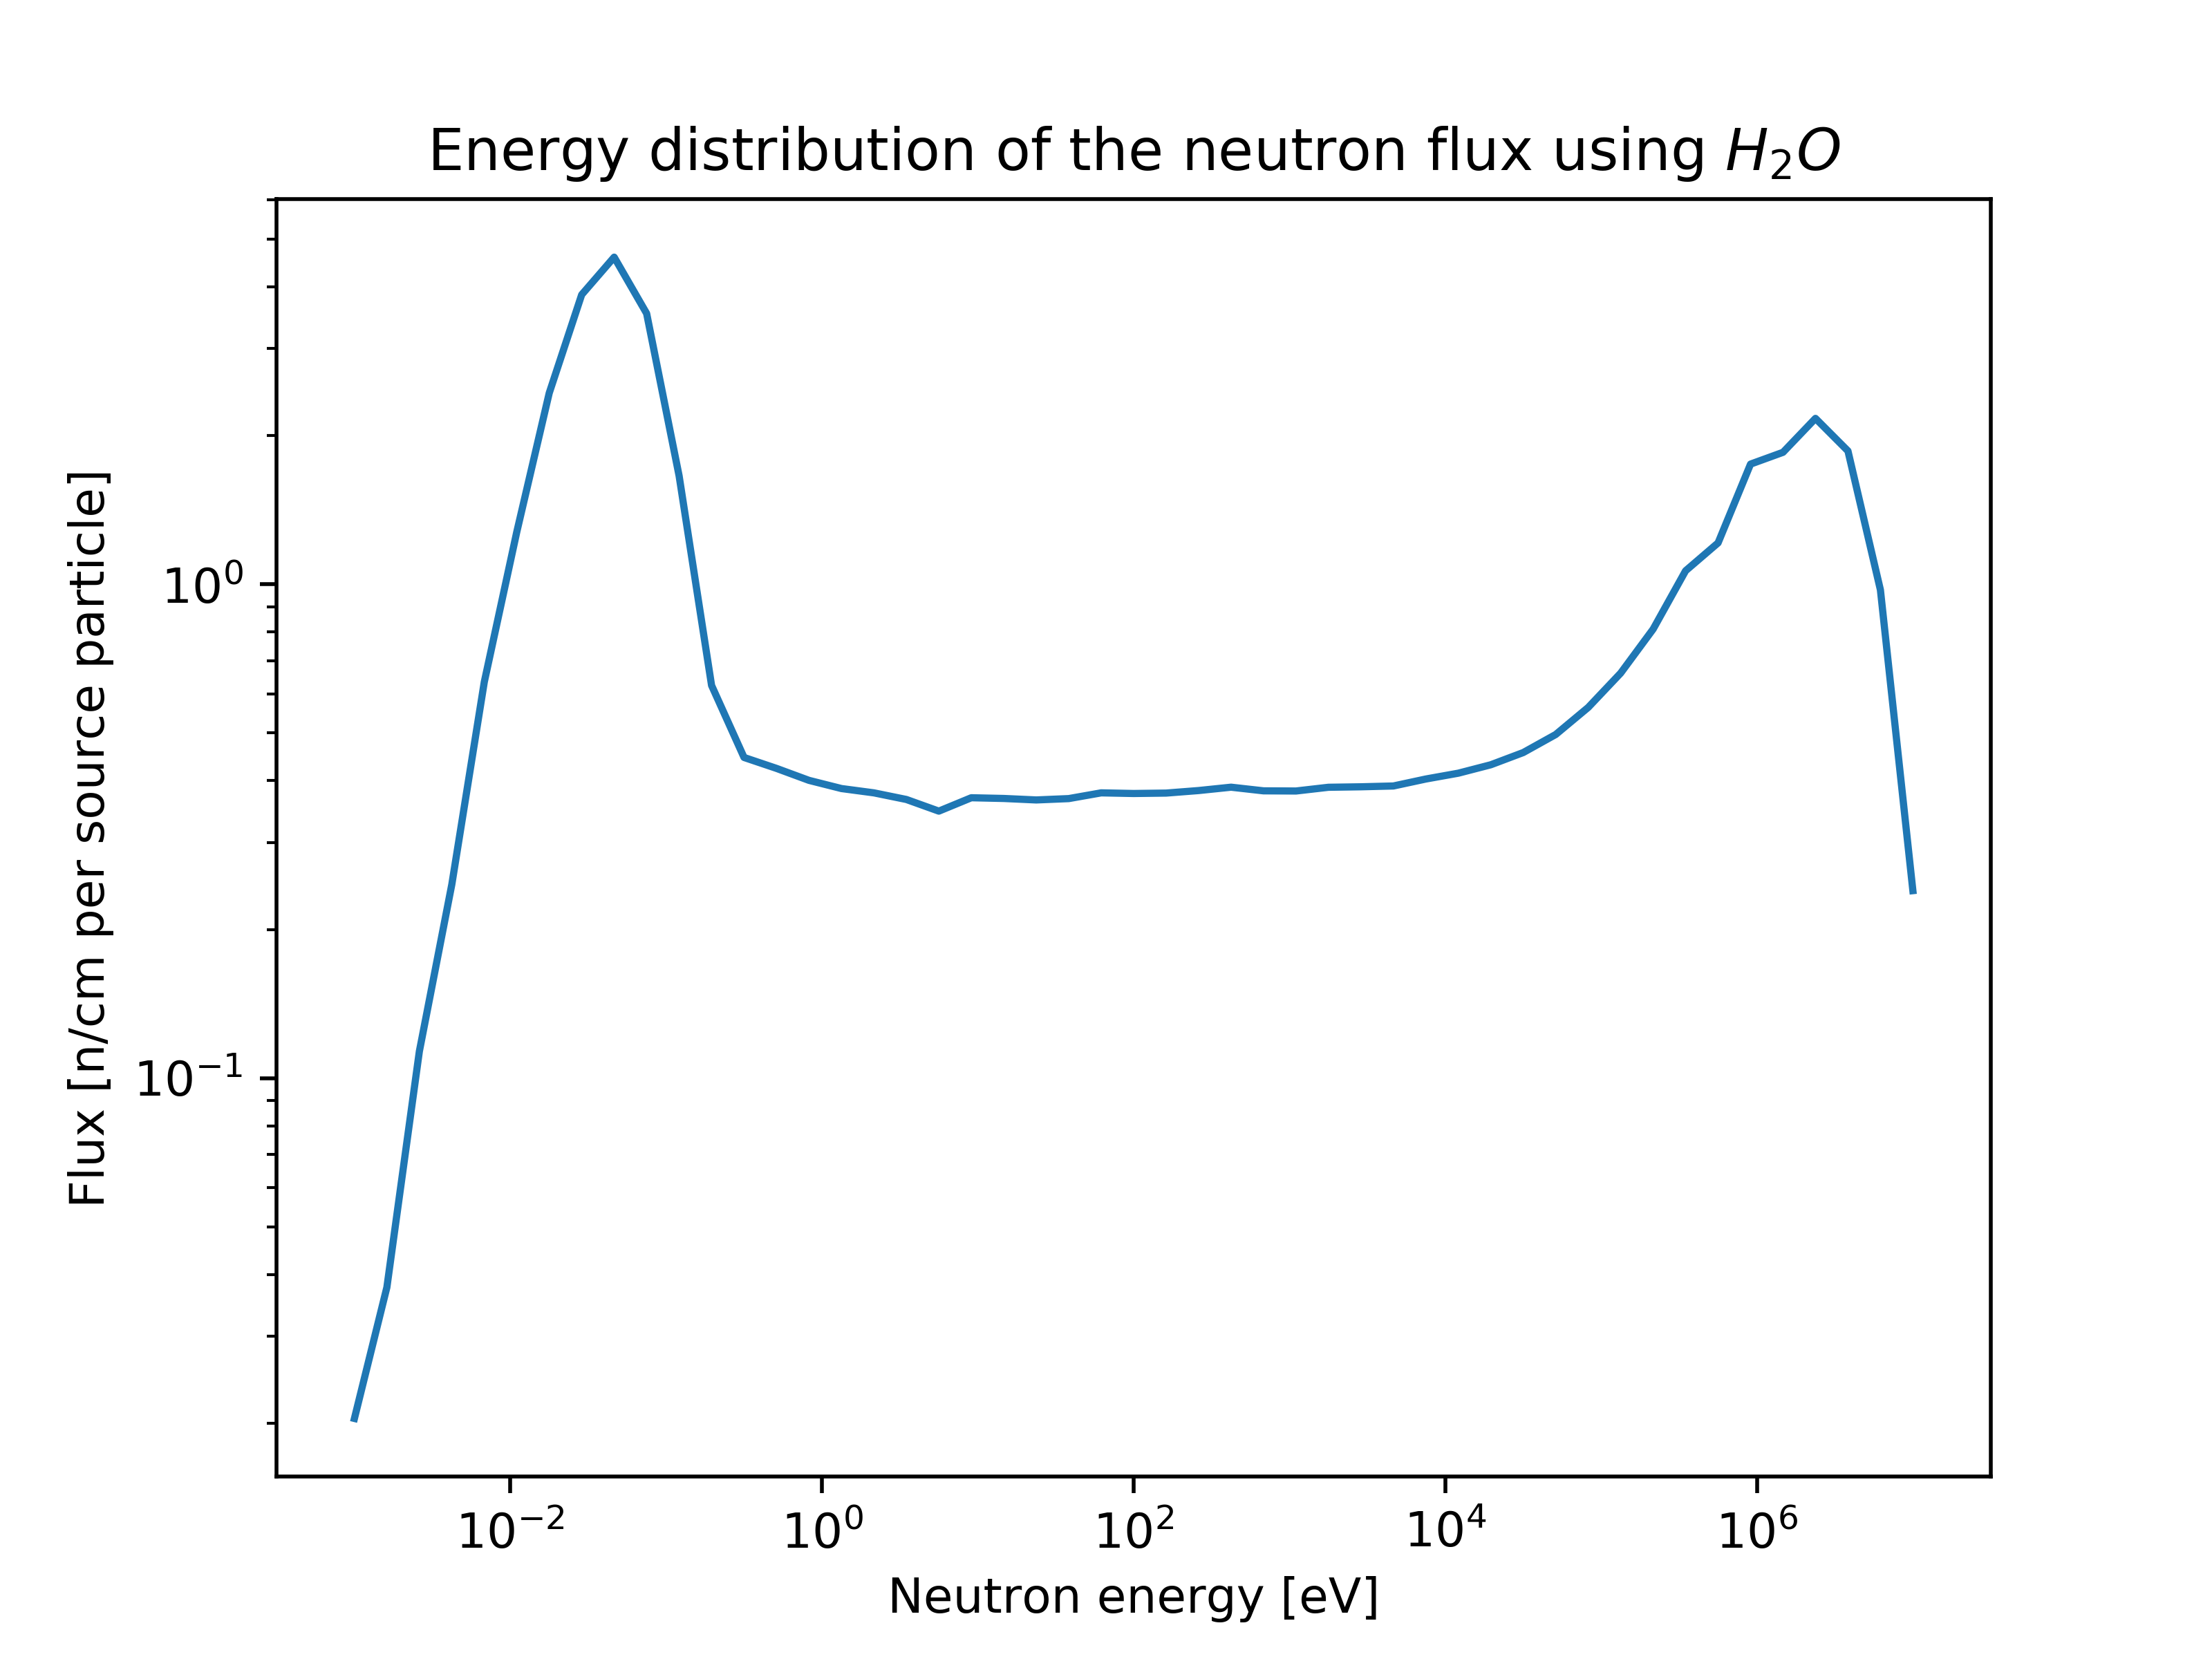
\includegraphics[width=0.5\textwidth]{energydistfluxh2o.png}
	\captionof{figure}{Energy distribution of the neutron flux using \ce{H_{2}O} as moderator.}
	\label{fig:fluxh2o}
	\end{center}
}


The moderator was changed when making the reactor go critical. Borated light water was used, where a boron concentration of $670$ ppm gave a criticality of $k_{\infty} = 0.99552 \pm 0.00117$. In nuclear power natural boron is used\cite{nuclear-power-boron}, so the \texttt{add\_element} function in OpenMC was used so that the natural isotopic composition of Boron was added in the moderator. Boron acts as a neutron absorber since $\ce{^{10}B}$ has a high (n,$\gamma$) cross-section for thermal neutrons. Since it absorbs thermal neutrons it lowers the thermal utilization factor $f$ in Eq. \ref{eq:kinfinity}. 

\multicolfloat{
    \begin{center}
	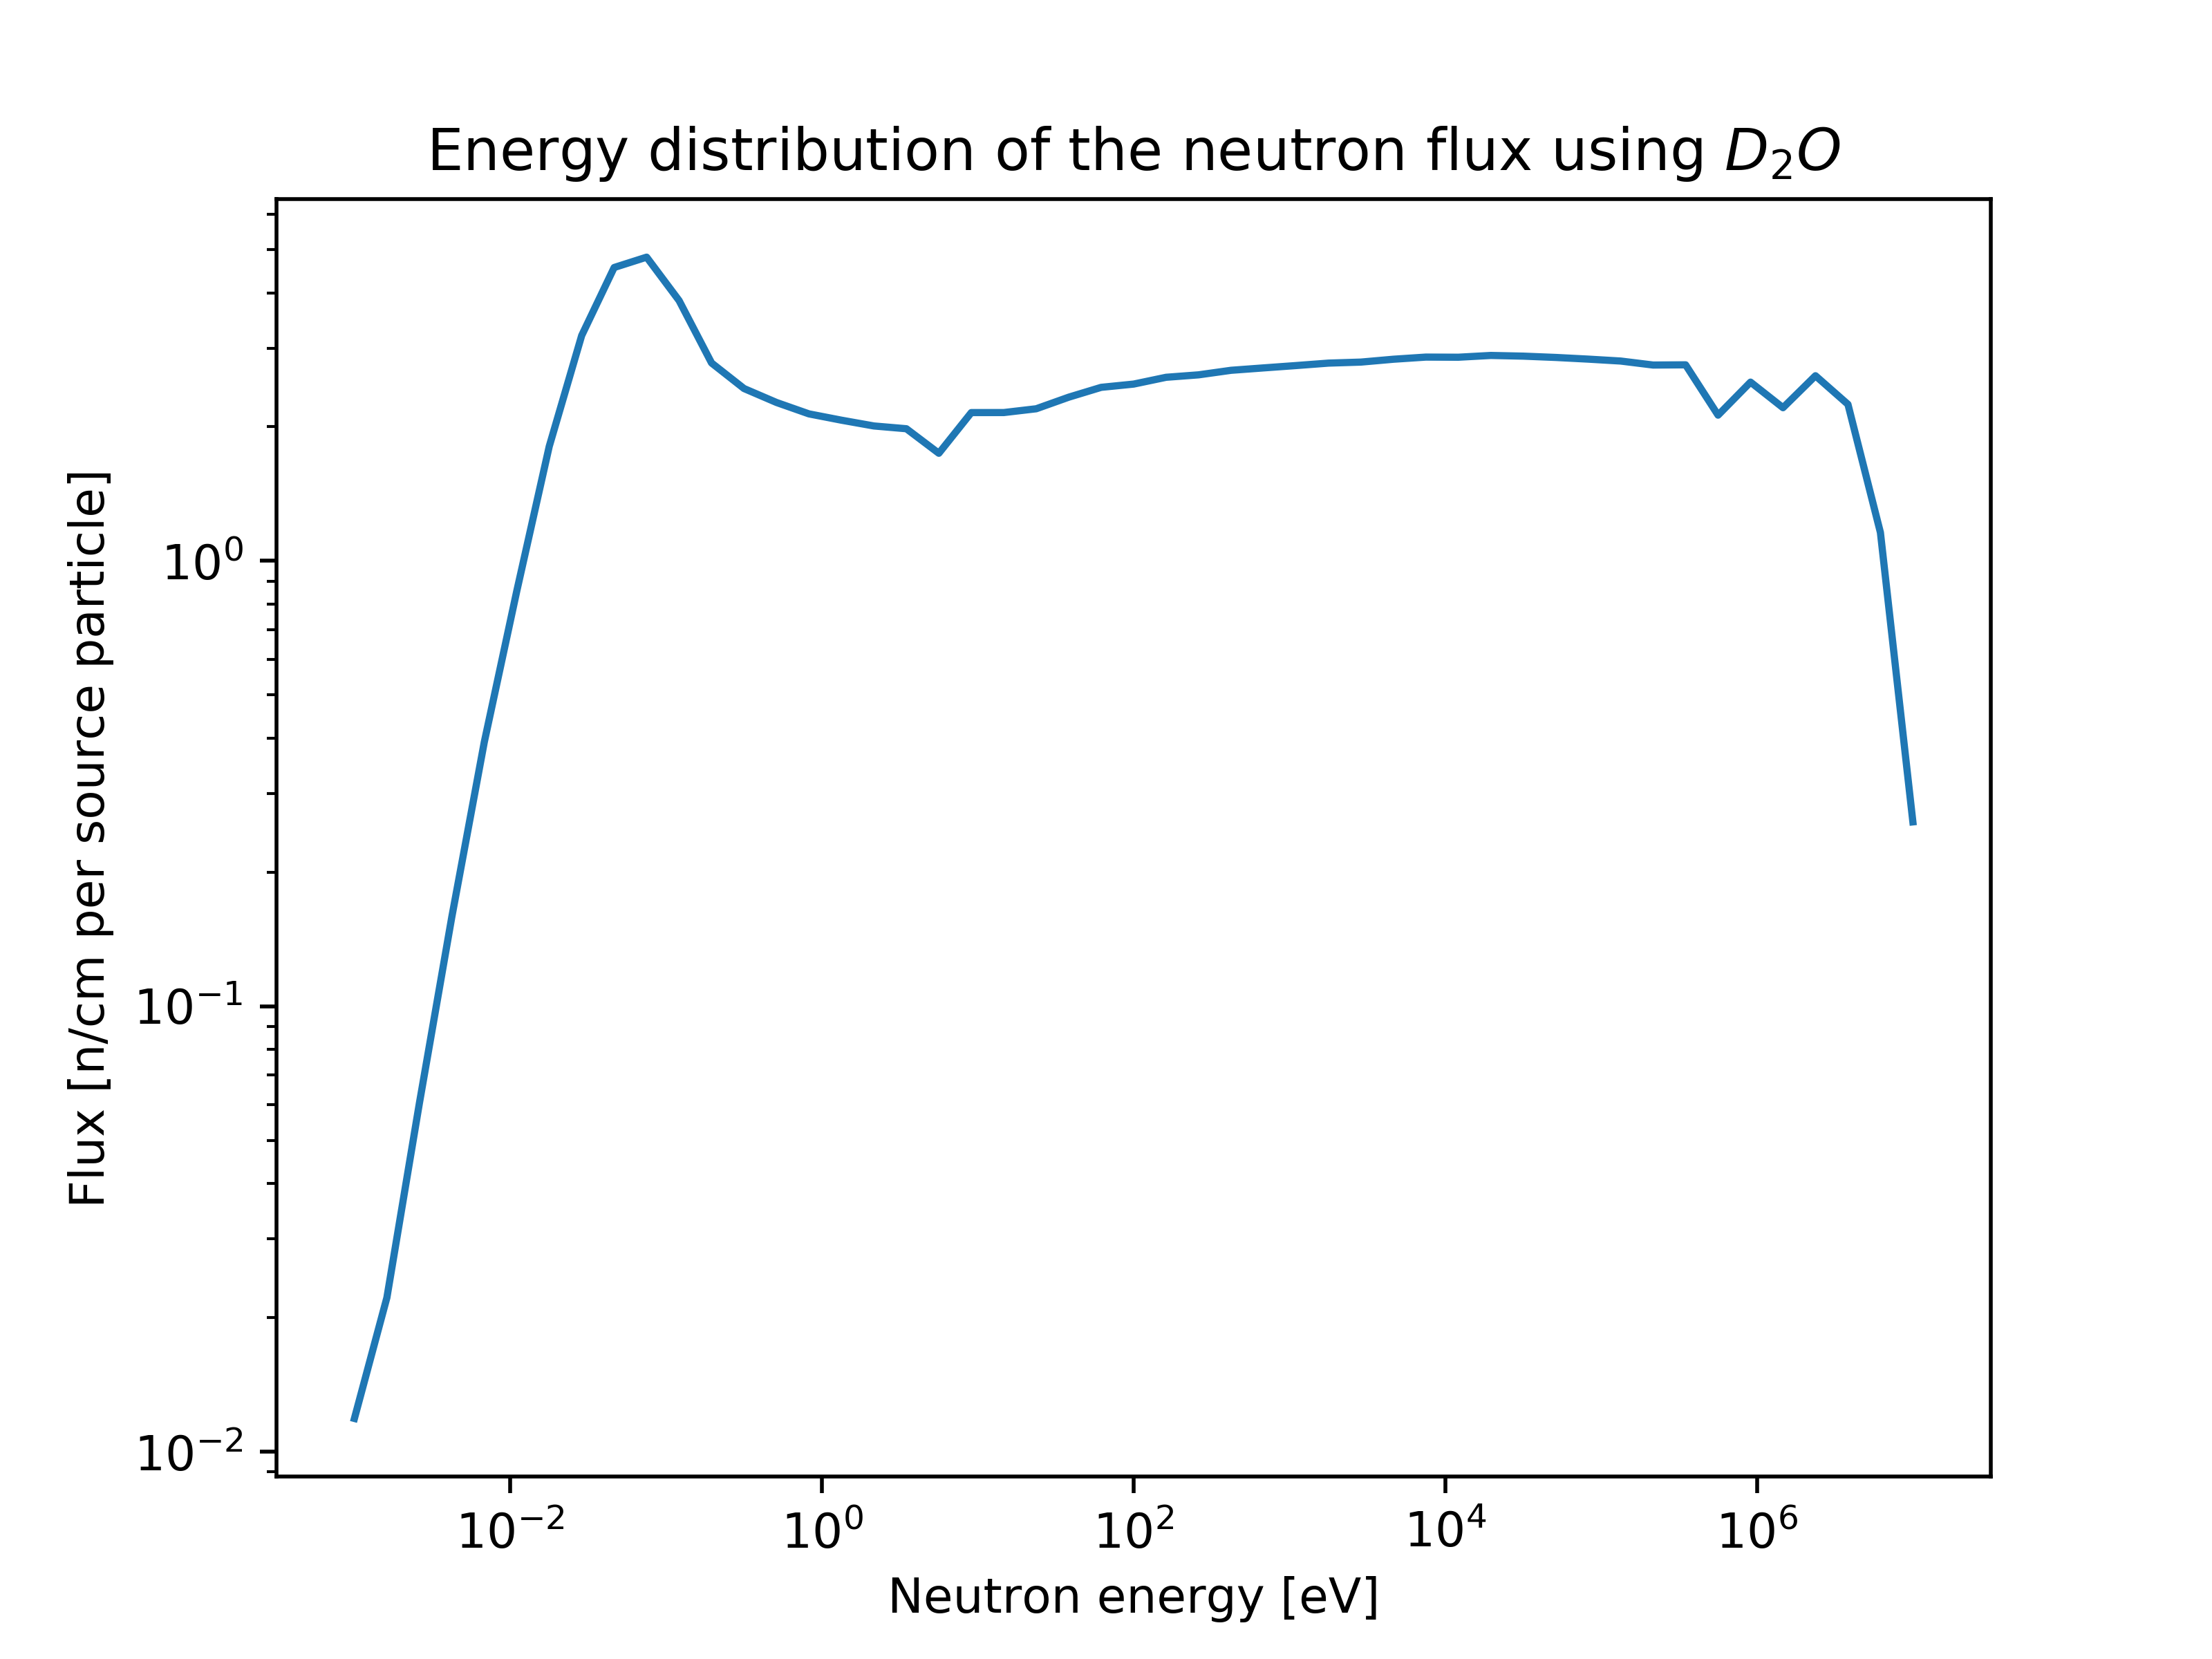
\includegraphics[width=0.5\textwidth]{energydistfluxd2o.png}
	\captionof{figure}{Energy distribution of the neutron flux using \ce{D_{2}O} as moderator.}
	\label{fig:fluxd2o}
    \end{center}
}


Increasing the void in the moderator is modelled by lowering the density of the moderator. This causes the criticality to increase, because the thermal utilization factor increases since there are voids where there is no boron to absorb the thermal neutrons.

The thermal utilization factor was calculated to be $0.59 \pm 0.02$ when looking at neutrons with energies from 0-0.025 eV.


\section{The Thorium Reactor}
This thorium reactor concept was inspired by the different fuel compositions made by the Norwegian company Thor Energy\cite{thorenergy}. Their thorium and plutonium mix, could help burning up existing plutonium waste from reactors. It could even help combat proliferation by burning weapons-grade plutonium. This is what has been modelled here, where a mixed oxide(MOX) consisting of 90$\%$ $\ce{Th}$ and 10$\%$ weapons-grade have been used. Weapons-grade plutonium consists of approximately $92\%$ $\ce{^{239}Pu}$ and $8\%$ $\ce{^{240}Pu}$\cite{worldnuclear}.

\multicolfloat{
    \begin{center}
	\includegraphics[width=0.5\textwidth]{fullcore10kpixels.png}
	\captionof{figure}{Image of the full reactor core. The different colors represent different materials. Black: shielding, grey: steel, cyan: borated water and pink: $\ce{Th}$ and $\ce{Pu}$ MOX fuel.}
	\label{fig:fullcore}
    \end{center}
}

A full core was built using a number of fuel assemblies of $10 \times 10$ fuel cells, as seen in Fig. \ref{fig:fullcore}. The details of the fuel cells become evident when looking at a smaller section of the core. From Fig. \ref{fig:zoomxy} the different parts of the cells are shown, i.e. the fuel material, the helium in the gap and the zirconium alloy cladding surrounding each cell. The water distributed around all the fuel rods is contains boron so that it absorbs neutrons, to avoid the reactor going super-critical. Each assembly also has a $2 \time 2$ sector in the center which is filled with moderator. These act as guide tubes for instrumental tubes or control rods, which can be inserted in these moderator-filled rods.


\multicolfloat{
    \begin{center}
	\includegraphics[width=0.47\textwidth]{zoom-xy-png.png}
	\captionof{figure}{Zoomed image of the reactor core, showing individual fuel cells. The pink is fuel, green is helium for gap, and brown is zirconium alloy cladding. The cyan between the cells is borated water.}
	\label{fig:zoomxy}
    \end{center}
}


To get the reactor critical boron was added to the $\ce{H_{2}O}$ moderator. A concentration of $25633.0$ ppm of natural (i.e. the natural abundance of isotopes) boron gave criticality of $k_{\text{eff}} = 0.99877 \pm 0.00129$. This was found running the OpenMC simulation using 5000 particles and 100 batches, where 8 of the batches were inactive. These settings are used throughout the thorium reactor simulations unless stated otherwise. The $k$ value found here is the $k_{\text{eff}}$ from Eq. \ref{eq:keff}, since this case is more realistic and does not have infinite (reflective) boundaries like the pin-cell, and therefore has leakage.

The effects of adding voids and/or increasing temperature was modelled by lowering the density of the borated water moderator. The expected results were a lower criticality, and even though that was what ended up happening, it was only lowered by a minuscule amount. It changed from $k_{\text{eff}} = 0.99877 \pm 0.00129$ to $0.97068 \pm 0.00140$ when lowering the density from $\rho = 0.740582$ $g/cm^2$ to $\rho = 0.440582$ $g/cm^2$. This is due to the fact that even if increasing voids and temperature would make for less moderator in the core and causing a lowered criticality, there is also a neutron absorber in the moderator, namely the boron. A lower density and less boron concentration in the core also ensures that fewer thermal neutrons are captured by boron. Therefore the change in criticality in this case is minimal. The effect of boron is also encountered when increasing the $\ce{H_2O}$ concentration in the moderator. $k_{\text{eff}}$ increases with higher $\ce{H_2O}$ concentration, as the relative amount of boron in the moderator then is lowered. When decreasing the $\ce{H_2O}$ concentration there is a higher neutron absorption and less moderation since the boron amount is relatively higher compared to $\ce{H_2O}$.

Such changes in e.g. temperature illustrates negative reactivity feedback, in that when a heating occurs and increases the power, there will be an automatic response from the reactor in that the density of the moderator decreases so that fewer neutrons in turn is thermalized, and then the power and criticality again returns to stability.

Figure \ref{fig:neutronfluxthorium} shows the energy distribution of the neutron flux. A comparison of this and Fig. \ref{fig:fluxh2o} would be natural, but here the difference is obvious. This is due to the fact that in the thorium reactor, boron is added to the moderator $\ce{H_{2}O}$ to act as a neutron absorber. Boron has a high cross section for neutron capture for thermal neutrons, and therefore the peak in the thermal region from Fig. \ref{fig:fluxh2o} has disappeared since the boron has absorbed these neutrons.

\multicolfloat{
    \begin{center}
	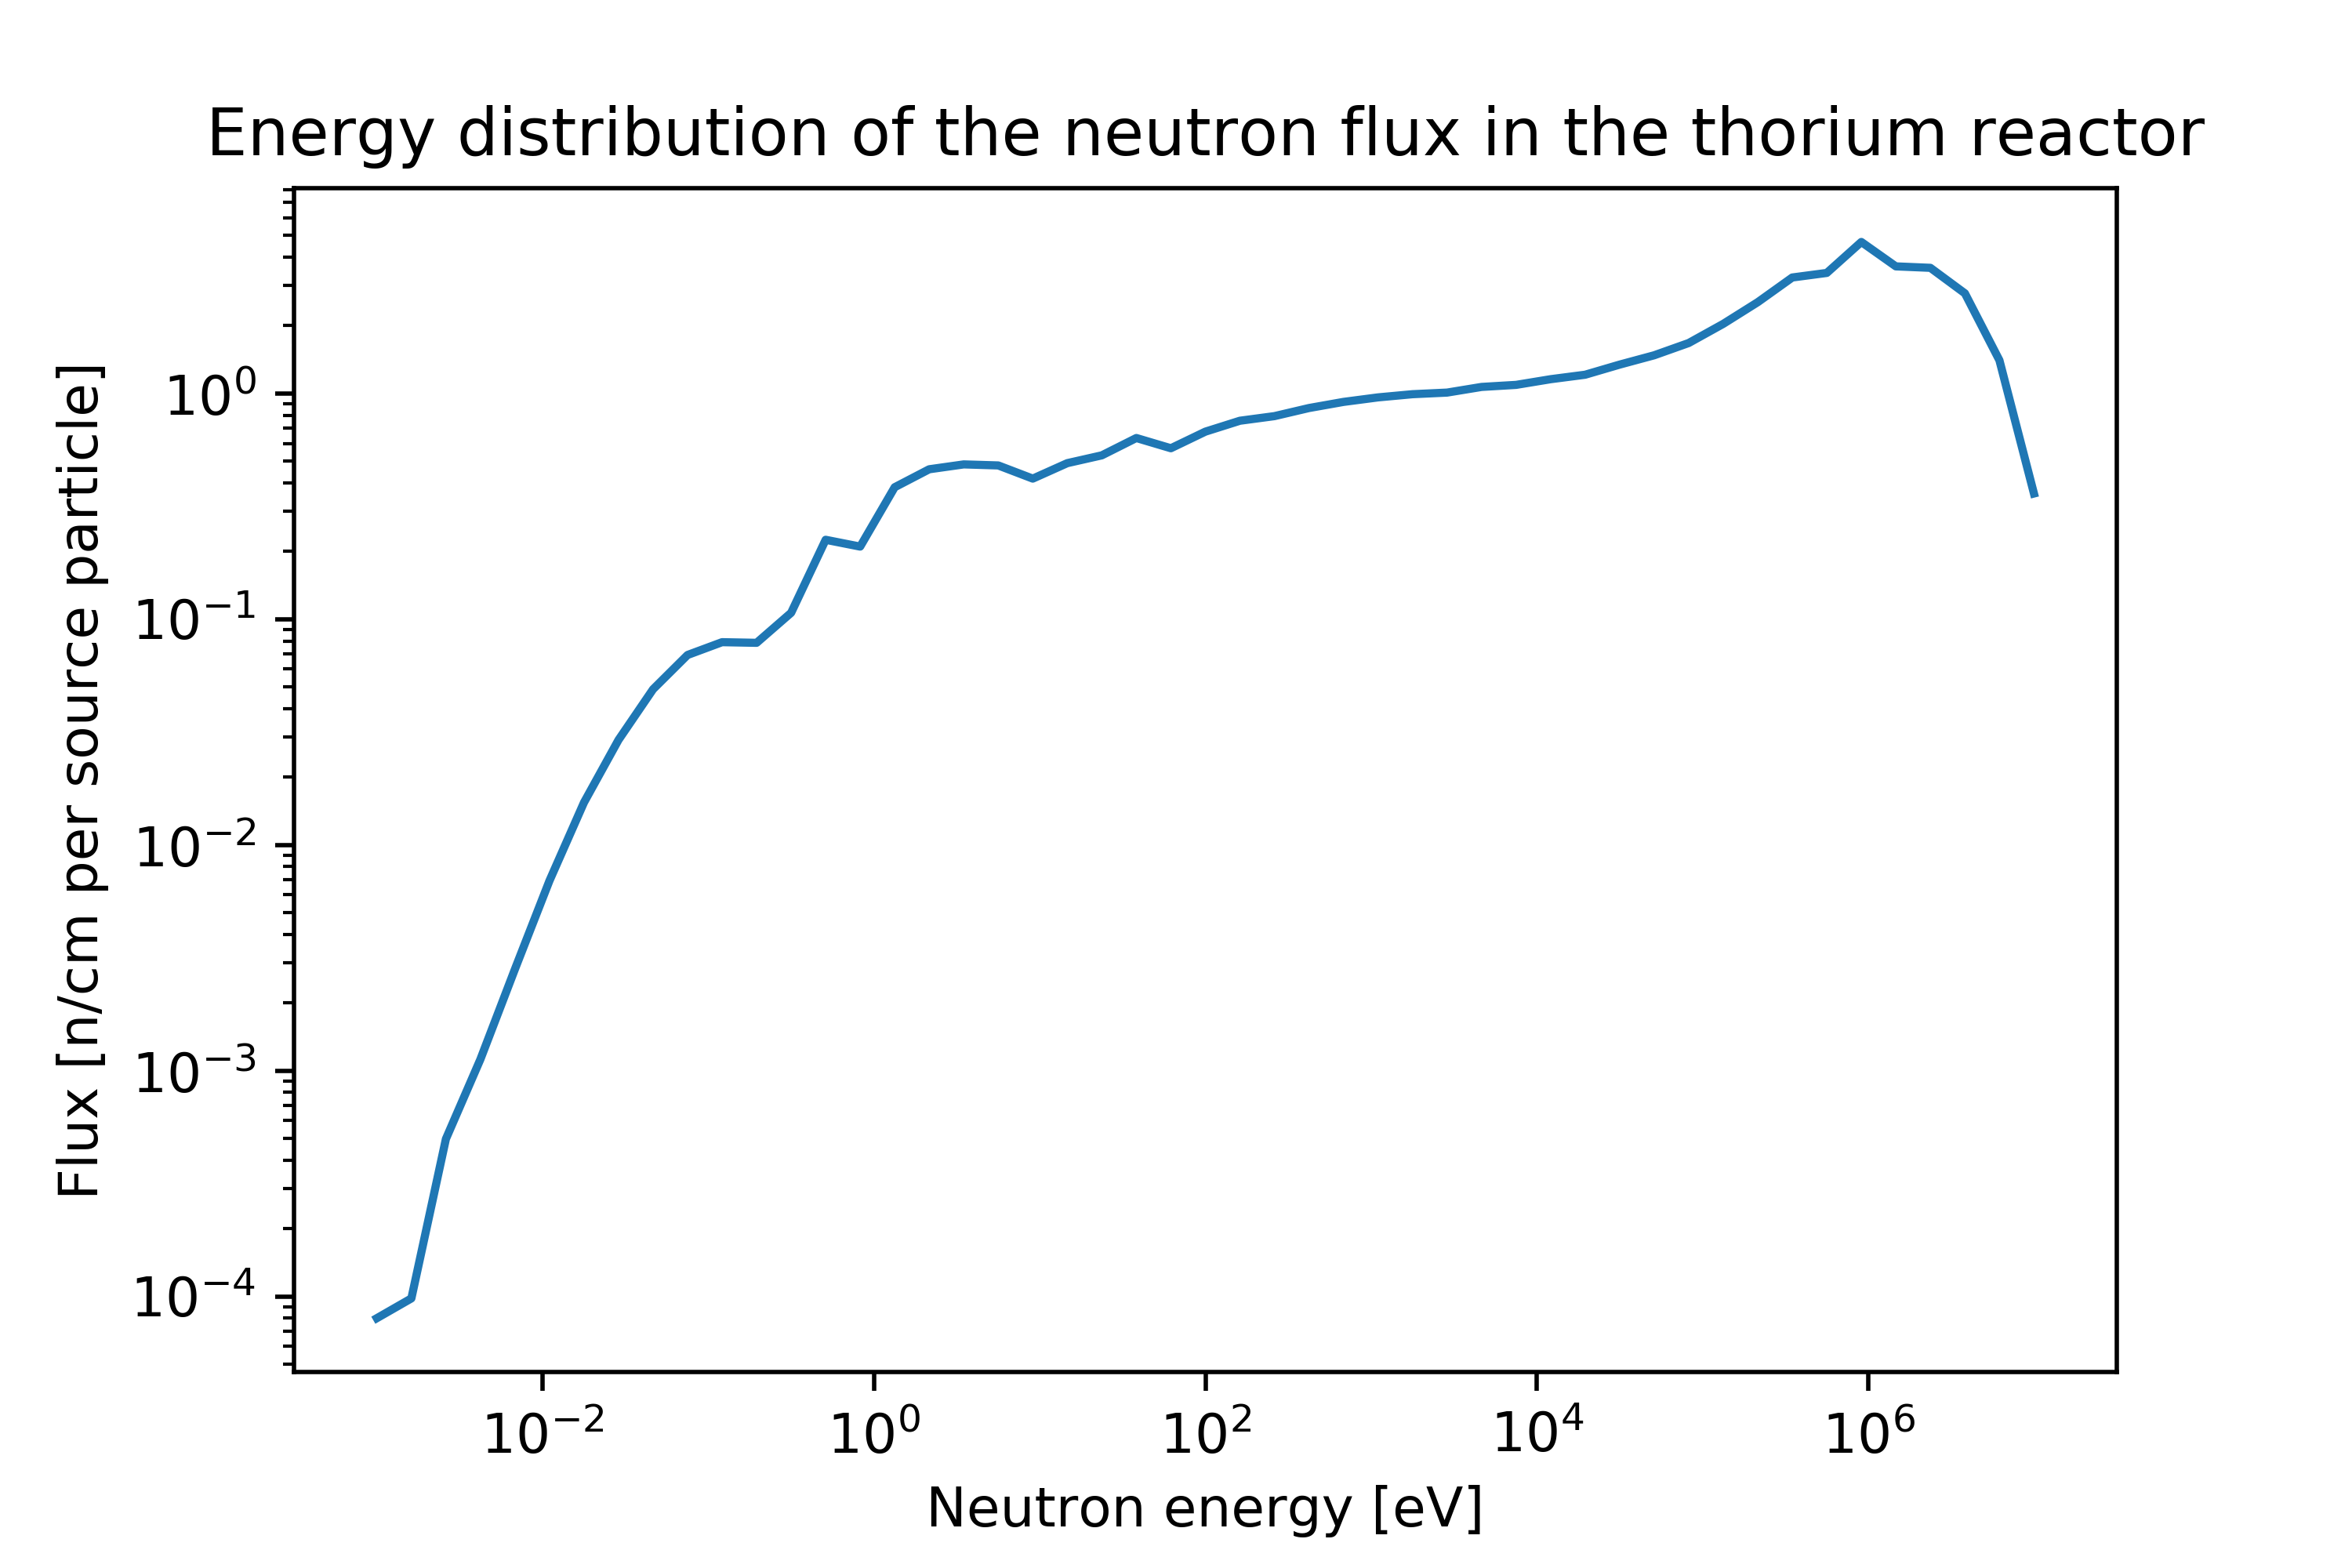
\includegraphics[width=0.5\textwidth]{neutronfluxdistthorium.png}
	\captionof{figure}{Energy distribution of the neutron flux using borated \ce{H_{2}O} as moderator.}
	\label{fig:neutronfluxthorium}
    \end{center}
}

The gamma flux energy distribution is included in Fig. \ref{fig:gammafluxthorium}. This was modelled using only 90 particles and 50 batches because of the amount of memory, storage and time it takes for computations when photon-transport is turned on in OpenMC.

\multicolfloat{
    \begin{center}
	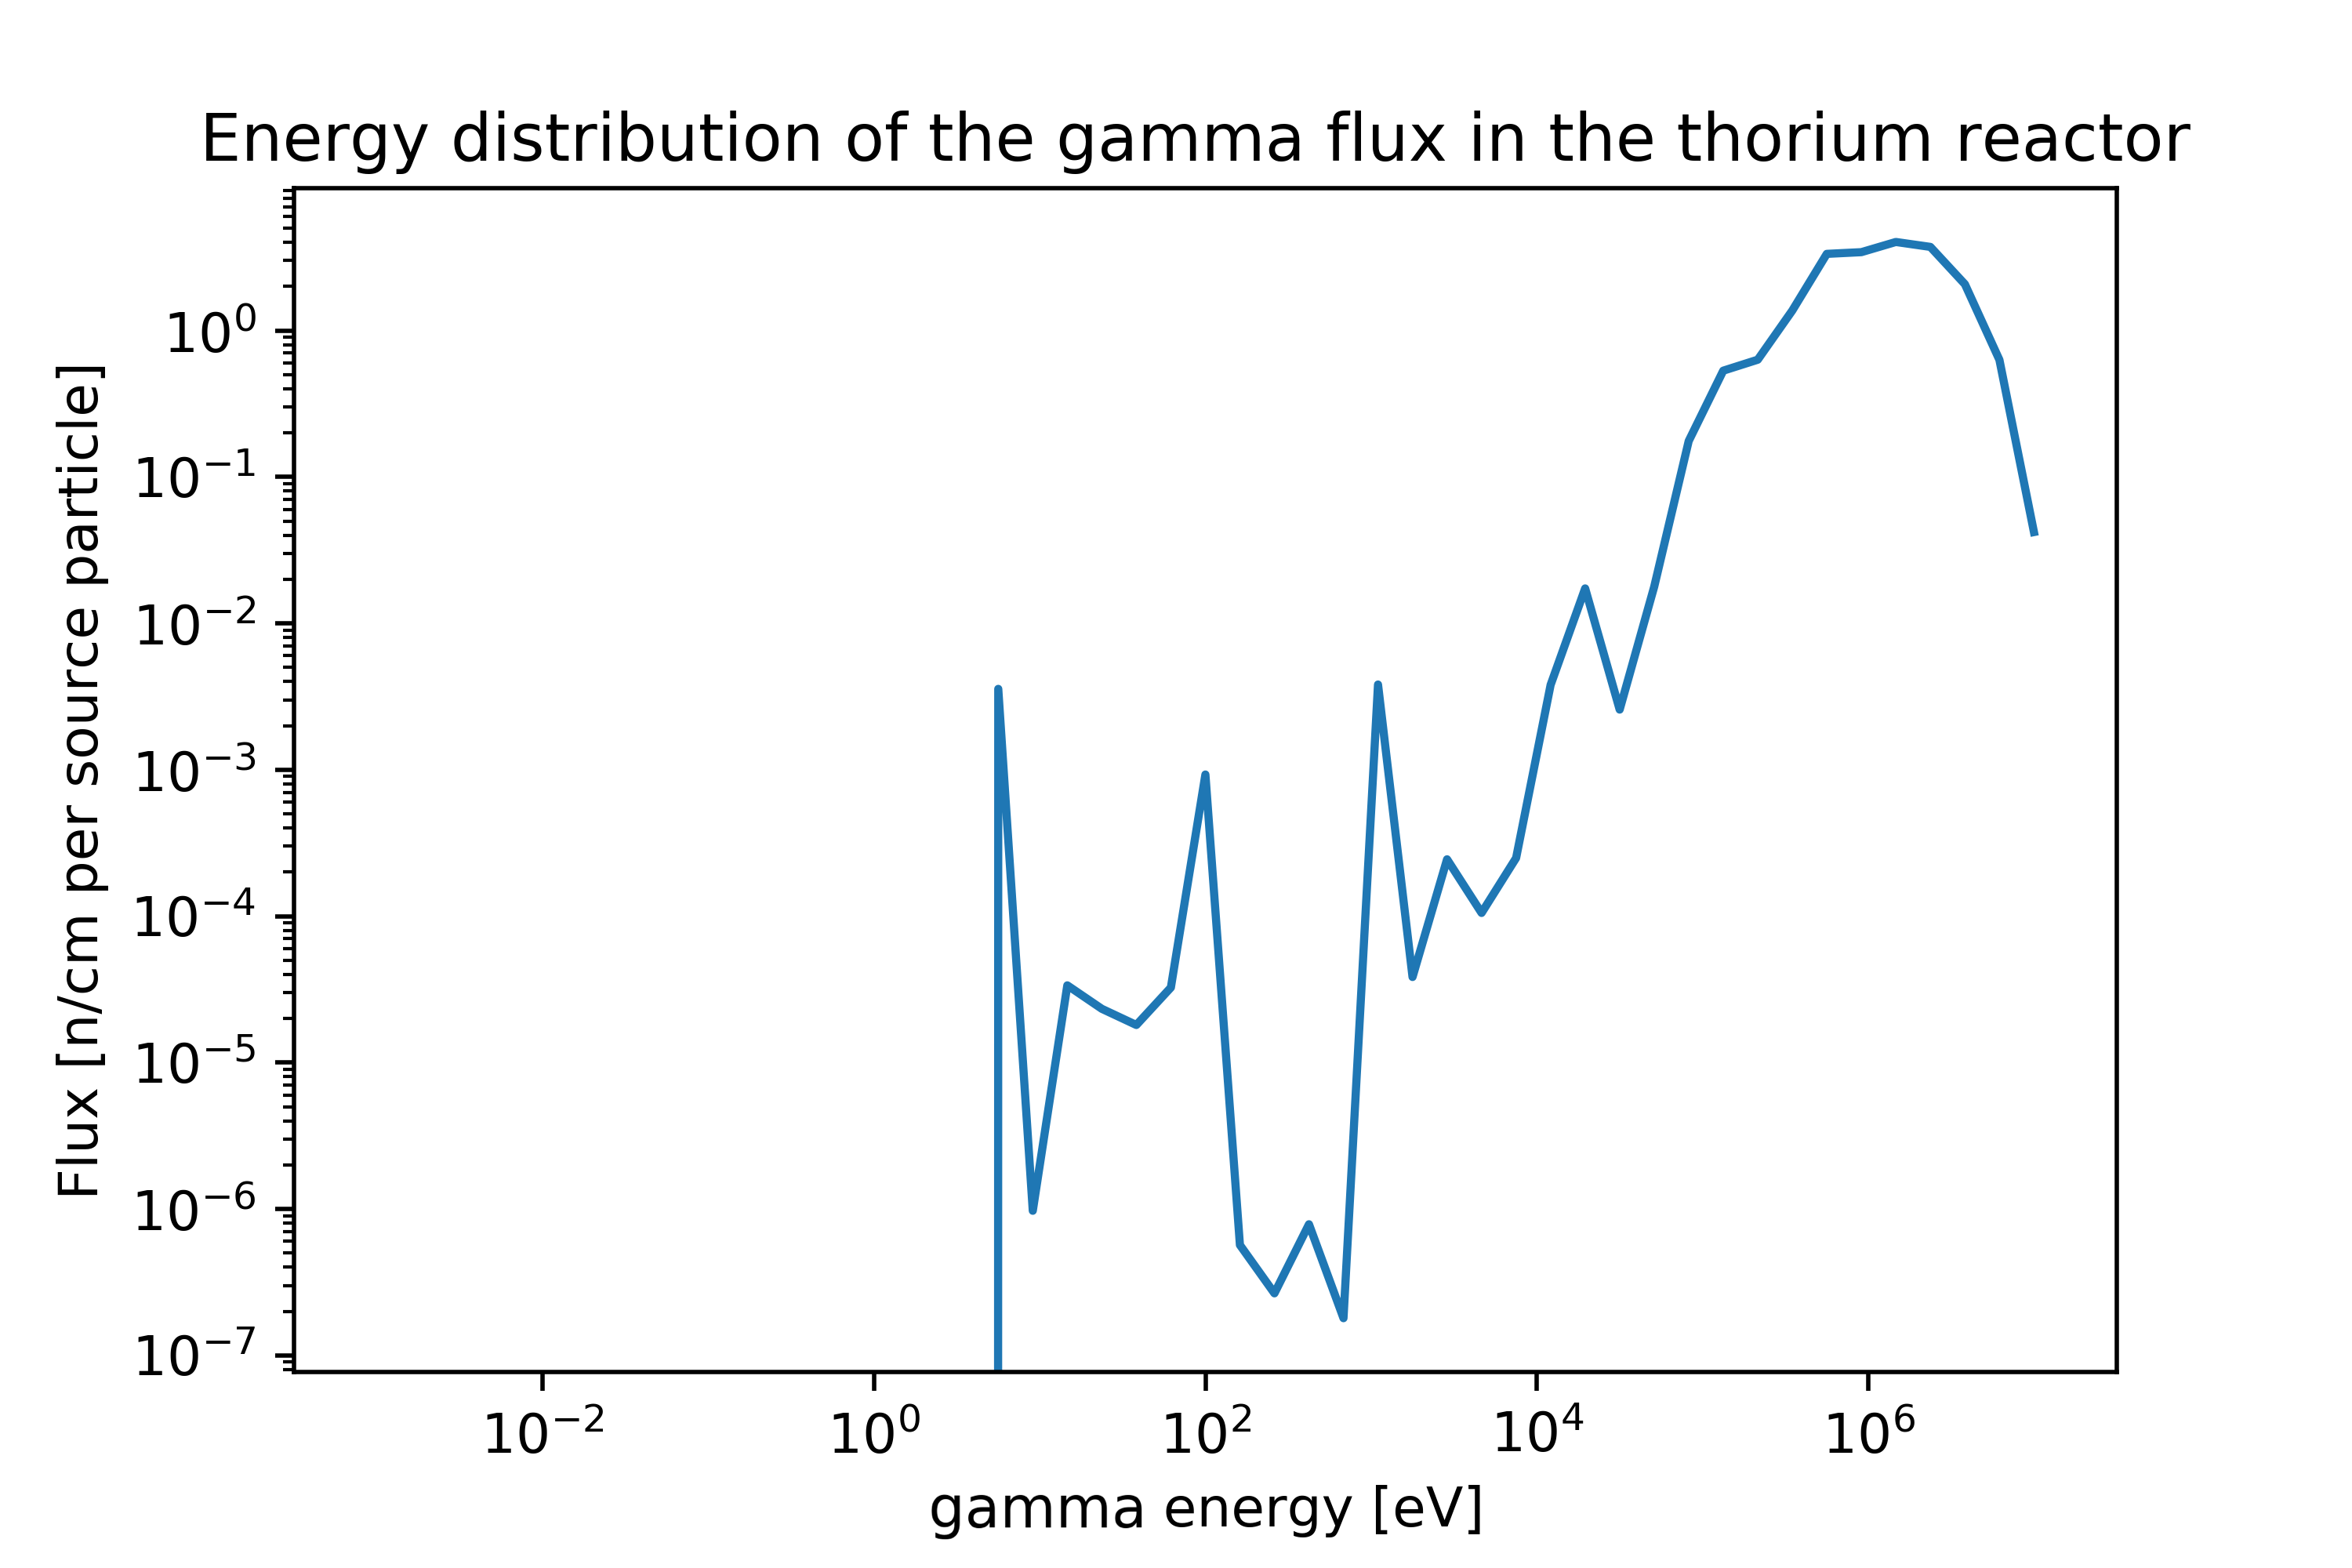
\includegraphics[width=0.5\textwidth]{gammafluxdistthorium.png}
	\captionof{figure}{Energy distribution of the gamma flux using borated $\ce{H_{2}O}$ as moderator.}
	\label{fig:gammafluxthorium}
    \end{center}
}

The thermal utilization factor of the reactor was also calculated, by looking at neutrons in the energy range of $0 - 0.05$ eV. This means that some of the neutrons investigated have energies a bit above the $0.025$ eV thermal energy, but is still included to look at a larger amount of low energy neutrons. The value of the utilization factor was found to be $f = 0.648703 \pm 0.008995$. 

\multicolfloat{
    \begin{center}
	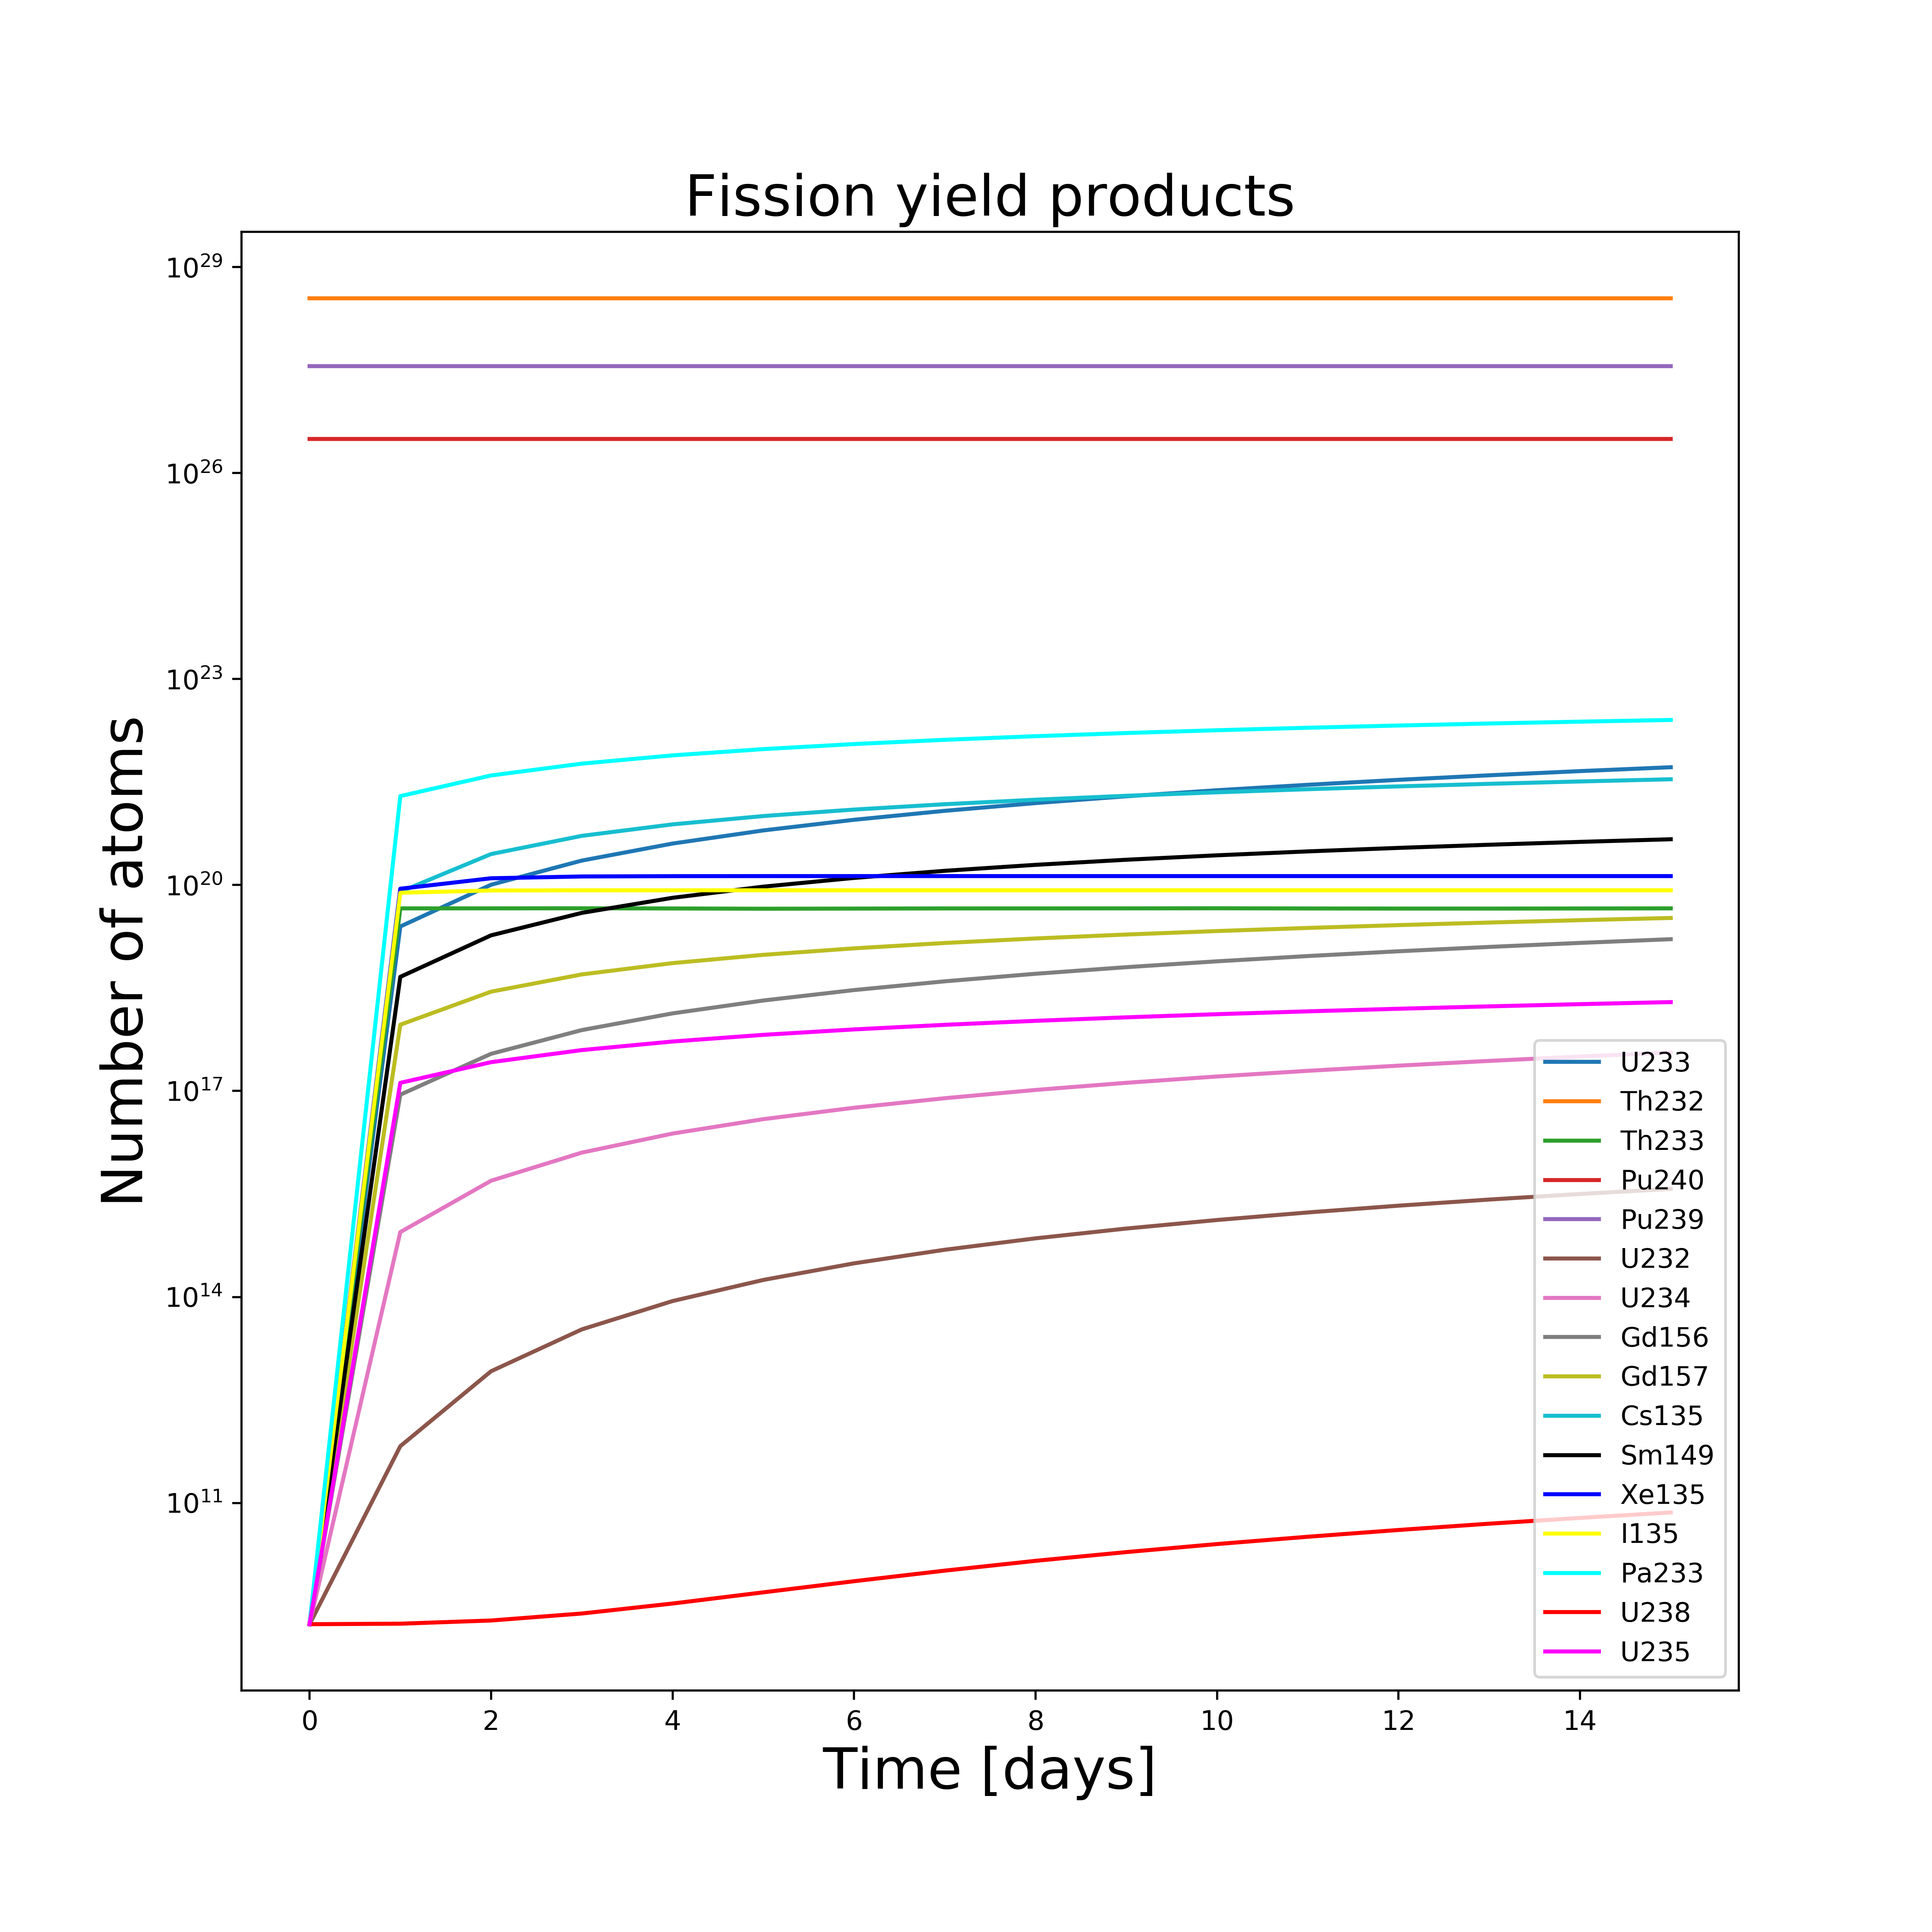
\includegraphics[width=0.5\textwidth]{fissionyieldproducts.png}
	\captionof{figure}{Fission yield products from running a 15 day depletion simulation.}
	\label{fig:fissionyield}
    \end{center}
}

A depletion simulation was ran with 1 day time-steps over a simulated 15 days. The depletion algorithm chosen was the \texttt{CF4Integrator} as outperformed the other algorithms with regard to numerical errors\cite{cf4paper} with a relatively short computation-time. A simplified depletion chain based on nuclides chosen by CASL-ORIGEN\cite{casl} was used with the depletion algorithm.

Some of the most important fission yield products produced are shown in Fig. \ref{fig:fissionyield}. There is a clear buildup of $\ce{^{233}U}$ which is the main product from the thorium, but also quite a few other uranium isotopes. This is due to the amount of plutonium included in the $\ce{ThO_2}$-$\ce{PuO_2}$ MOX fuel. In this simulation the initial fuel is constant. The buildup of uranium isotopes would increase the criticality, but there is also a buildup of different neutron poisons like $\ce{^{135}Xe}$ and $\ce{^{149}Sm}$ which counteracts this. Therefore the criticality is quite constant around $k_{\text{eff}} \approx 1.0$, as is seen in Fig. \ref{fig:keffdepletion} 

\multicolfloat{
    \begin{center}
	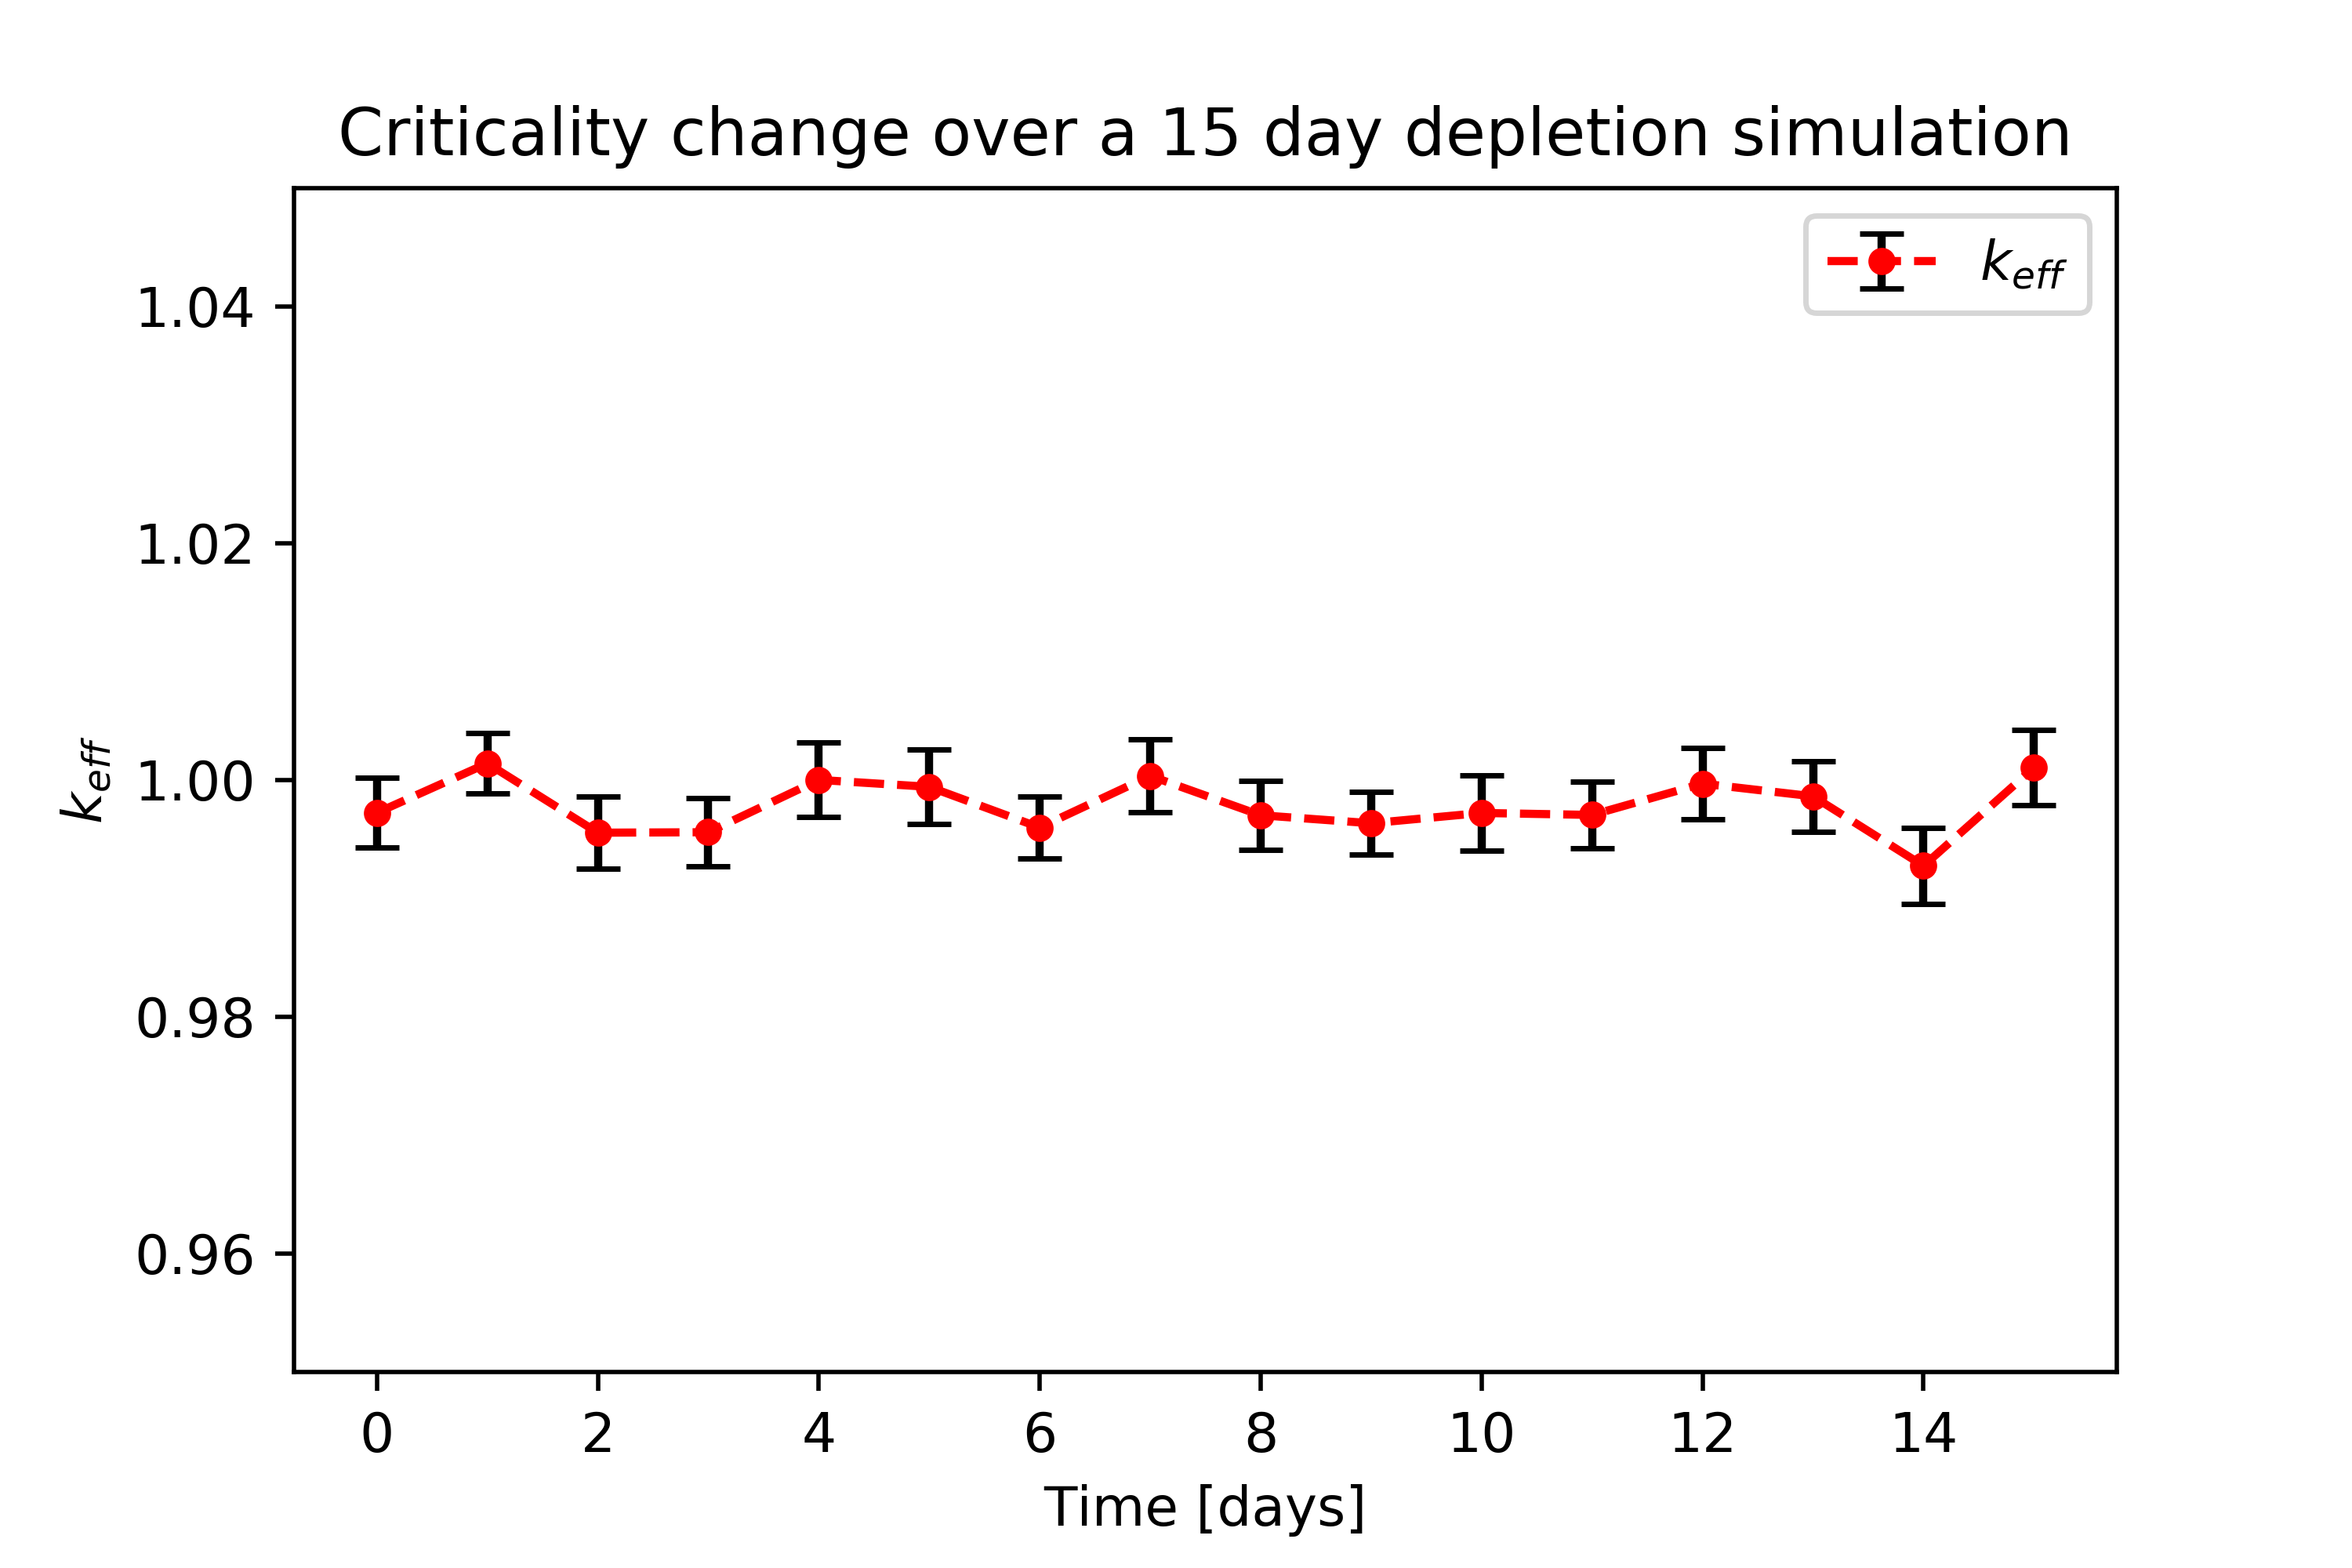
\includegraphics[width=0.5\textwidth]{keff-depletion.png}
	\captionof{figure}{$k_{\text{eff}}$ variations over a 15 day depletion simulation.}
	\label{fig:keffdepletion}
    \end{center}
}

The amount of neutrons absorbed by the neutron poisons $\ce{^{135}Xe}$ and $\ce{^{149}Sm}$ is shown in Fig. \ref{fig:absorption}.

\multicolfloat{
    \begin{center}
	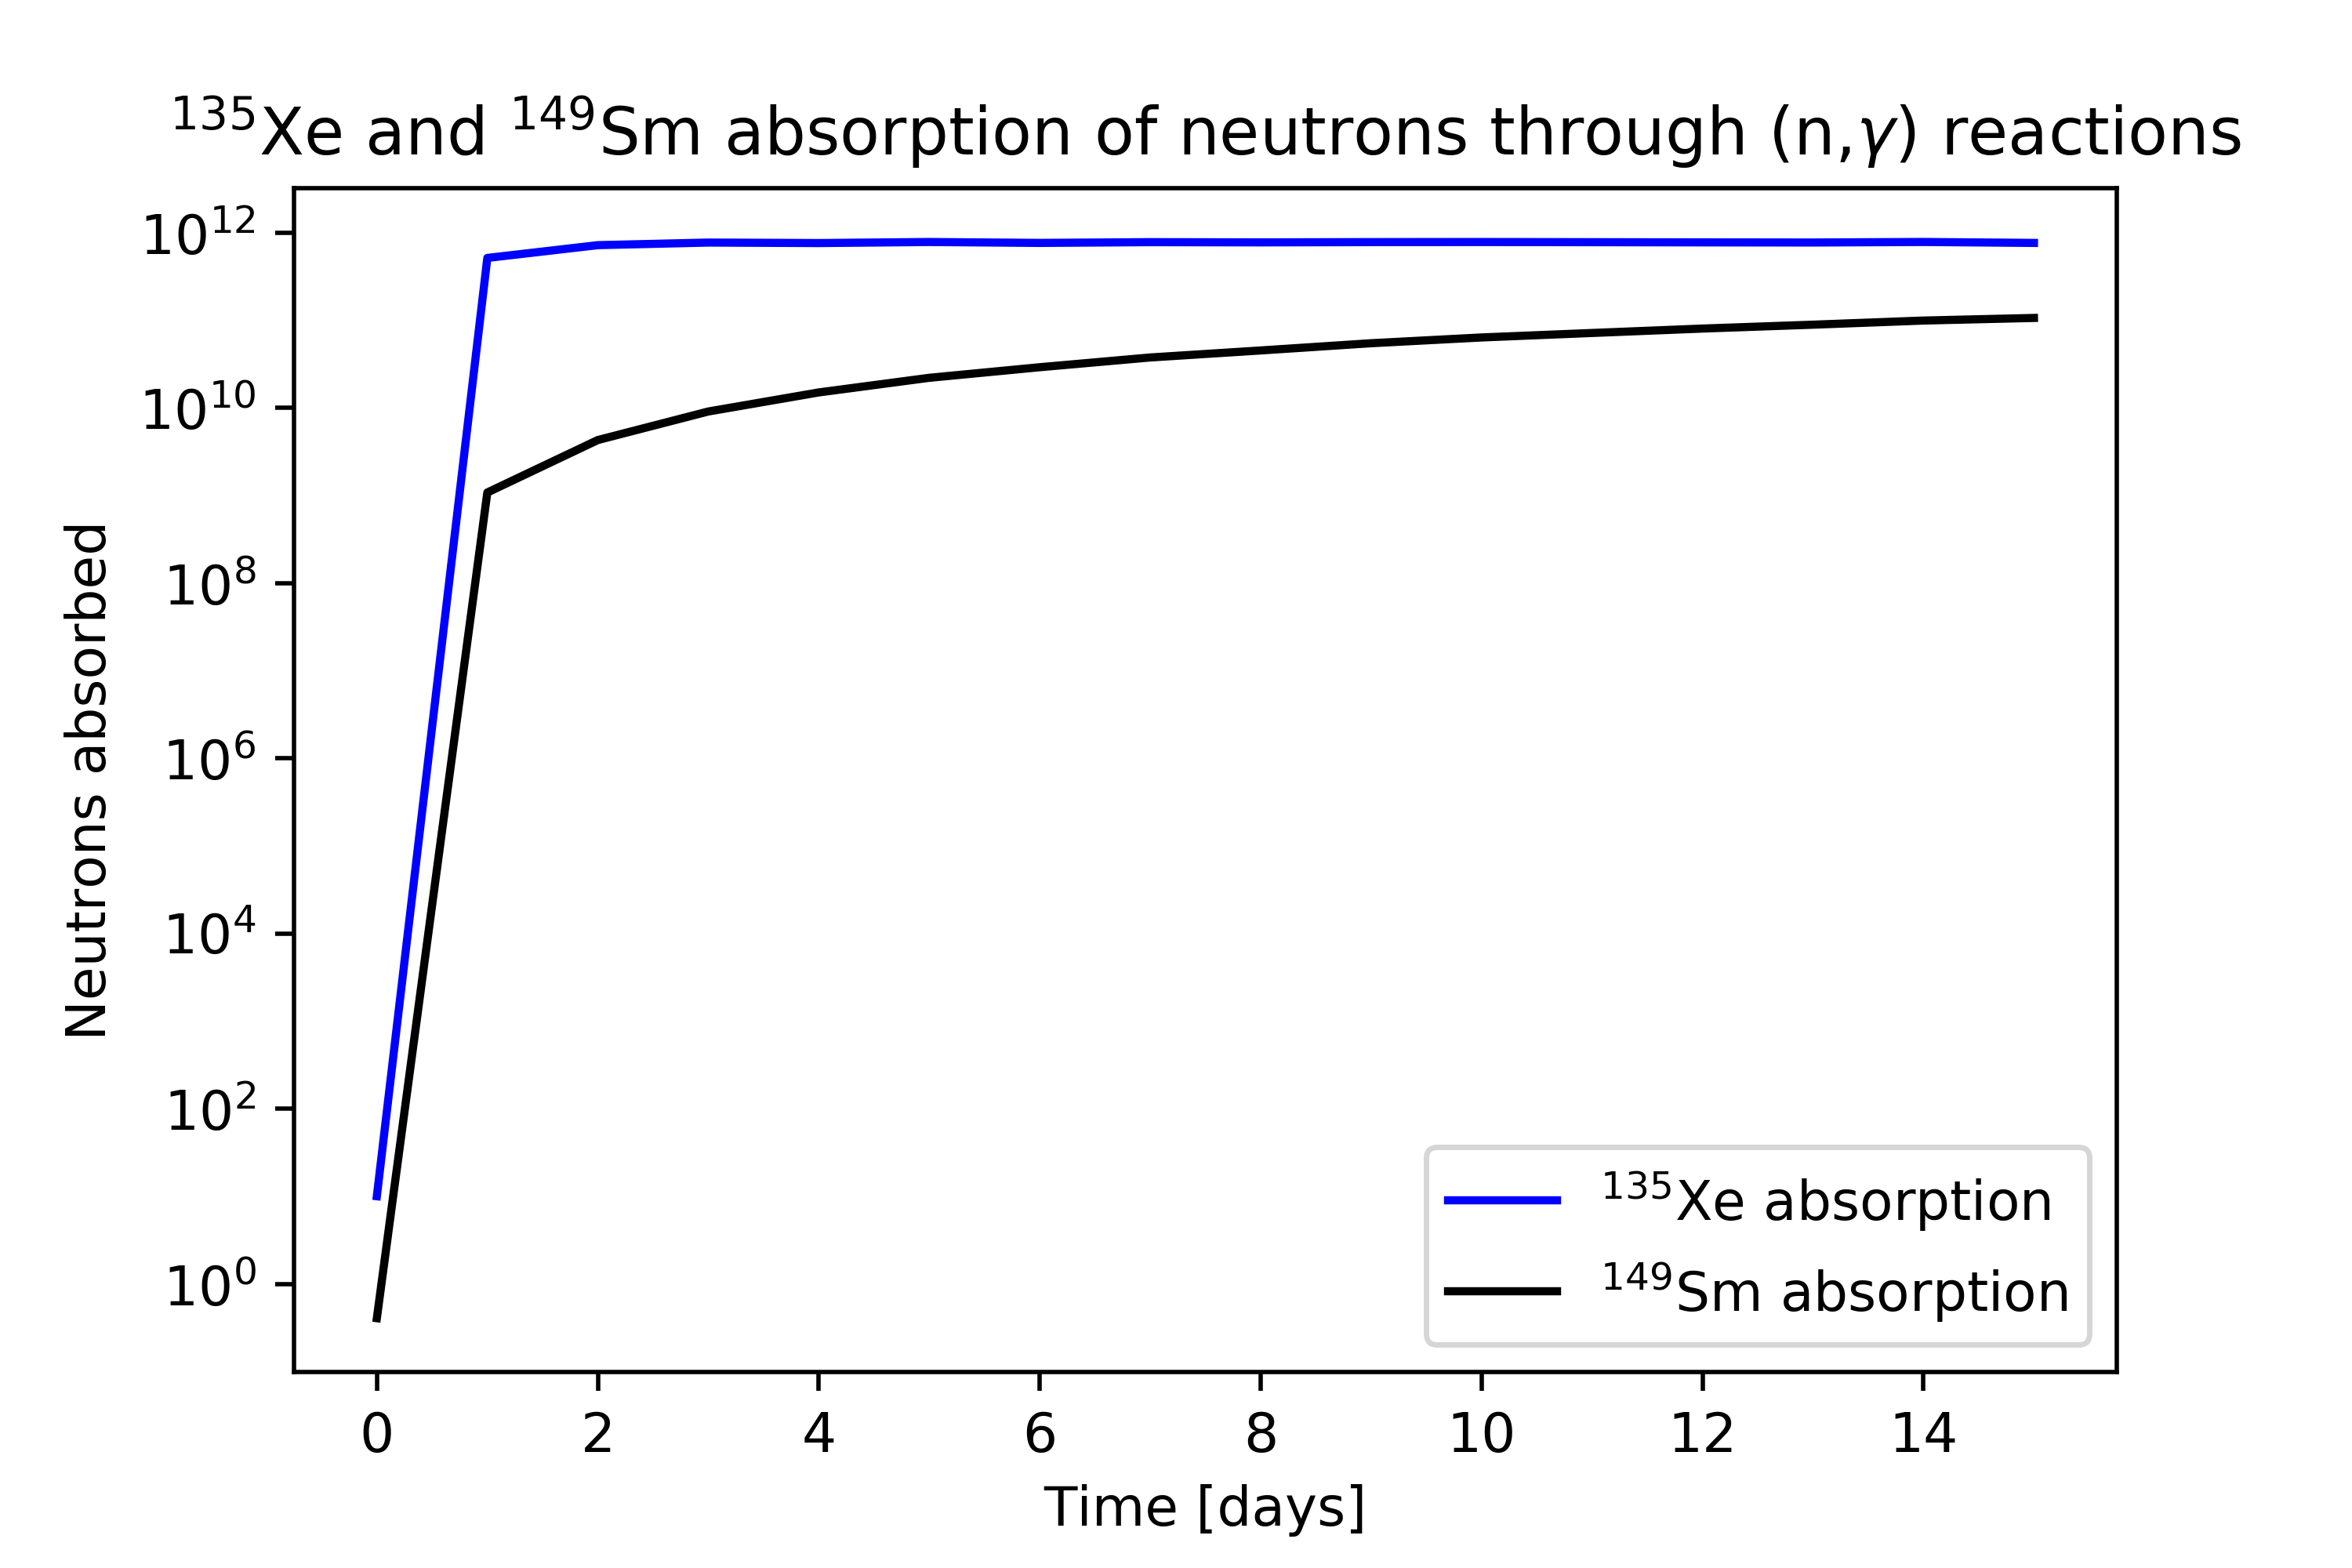
\includegraphics[width=0.5\textwidth]{xe135sm149absorption.png}
	\captionof{figure}{The amount of neutrons absorbed by the $\ce{^{135}Xe}$ and $\ce{^{149}Sm}$ neutron poisons.}
	\label{fig:absorption}
    \end{center}
}

\section{Discussion}

Thorium reactors have many advantages compared to traditional uranium-plutonium based reactors\cite{nuclpowerthorium}. The natural abundance of thorium on earth being one of them. There is about three times as much thorium as there is uranium in the earth's crust, and nearly all natural thorium is $\ce{^{232}Th}$ so no enrichment is needed. In thermal reactors thorium also has a larger reproduction factor than uranium-based fuel. 
\\
There are also advantages that could help sway the politicians towards thorium reactors. The general consensus is that thorium-based fuels are more proliferation resistant than uranium reactors. Part of this is because of the lower production of transuranic elements in the thorium cycle. Another advantage that has been investigated in this work is the fact that weapons-grade (and reactor-grade) plutonium can be used as fuel, and burnt up. 

Possible disadvantages include the fact that the delayed neutron fraction is lower for $\ce{^{133}U}$ than $\ce{^{235}U}$, and thus it is harder to control the reactivity using delayed neutrons. Another issue is the fact that $\ce{^{232}U}$ decay produces very penetrating and dangerous $\gamma$-rays. The decay-chain from fertile $\ce{^{232}Th}$ into $\ce{^{233}U}$ includes the $\beta^-$-decay of $\ce{^{233}Pa}$ into $\ce{^{233}U}$. $\ce{^{233}Pa}$ has a half-life of approximately 27 days. The problem then is that $\ce{^{233}Pa}$ has a significant neutron absorption cross section, and to avoid $\ce{^{233}Pa}$ "stealing" more neutrons and lowering the neutron economy it needs to be isolated to reduce neutron capture.

Breeding reactors like the one simulated here also have additional requirements. They need a conversion(breeding) ratio above $1.0$. The conversion ratio can be described as
\begin{equation*}
    \text{\small{conversion ratio}} = \frac{\text{\small{fissile isotopes created}}}{\text{\small{fissile isotopes destroyed}}}
\end{equation*}
To achieve a conversion rate larger than 1 an excess of neutrons is essential, and $\eta - 1$ needs to be as large as possible. A high neutron flux throughout the reactor is thus required. In the thermal region $\ce{^{233}U}$ has the highest reproduction factor, $\eta$, so therefore thorium fuel make for good breeding reactors.


\section{Conclusion}
Different aspects of reactor physics have been discussed by simulating both a simple pin-cell reactor and a more complex thorium breeder reactor setup. The pin-cell illustrated many issues that could be encountered when designing a reactor fuel cell, such as cell area compared to moderator area, which proved the point that heavy water generally is a better moderator than light water, but that it does indeed need a higher number of collisions to moderate the neutrons from the fast to the thermal region. Different resonance peaks in the neutron flux was also found when comparing $\ce{H_2O}$ and $\ce{D_2O}$. 

In the thorium breeder reactor a $\ce{ThO_2}$-$\ce{PuO_2}$ MOX was used as fuel. The moderator was regular light water with a boron concentration of $25633.0$ ppm. This achieved a criticality of $k_{\text{eff}} = 0.99877 \pm 0.00129$. 
\\
From running a depletion chain and investigating what happened in the reactor over time, it was evident that the reactor maintained its criticality. A reactor like this, which could burn up both reactor-waste grade and weapons-grade plutonium would seem like a very appealing choice. It could help both reduce the dangerous waste from older reactors, in addition to help the ongoing proliferation reduction. 

The Norwegian company Thor Energy\cite{thorenergy}, whose fuel composition is what this reactor was based on, have made several attempts to utilize the thorium in the Norwegian crust. As the demand of clean $\ce{CO_2}$ free energy increases with the ongoing environmental concerns, the Norwegian government should invest more funds into researching a possible thorium reactor. Norway has one of the largest thorium concentrations in the world\cite{thorium2008}, and if this could be exploited it could both help supply the country with energy, in addition to help Norway keep exporting and selling energy across Europe. 


\bibliography{References}

\begin{thebibliography}{999}

\bibitem{openmc}
Paul K. Romano, Nicholas E. Horelik, Bryan R. Herman, Adam G. Nelson, Benoit Forget and Kord Smith, \textit{OpenMC: A State-of-the-Art Monte Carlo Code for Research and Development}, Ann. Nucl. Energy, 82, 90–97 (2015).

\bibitem{githubjulian}
GitHub directory containing the codes used in this project. \href{https://github.com/jvevik/FYS4580}{https://github.com/jvevik/FYS4580}.


\bibitem{sindrehk}
GitHub-link to the scripts made by Sindre Hestnes Kaald for the course FYS4580 at the University of Oslo, Fall 2019. \href{https://github.com/sindrehk/FYS4580}{https://github.com/sindrehk/FYS4580}


\bibitem{stacey}
Stacey, Weston M. \textit{Nuclear Reactor Physics}. 2nd ed., completely rev. and enl. ed., Wiley-VCH, 2007.

\bibitem{nuclear-power-boron}
Nuclear-power.net, \textit{Applications of Boron - Nuclear Power}, \href{https://www.nuclear-power.net/glossary/boron-10/applications-of-boron-nuclear-power/}{https://www.nuclear-power.net/glossary/boron-10/applications-of-boron-nuclear-power/} (Accessed 26.10.19).

\bibitem{thorenergy}
Thor Energy. Homepage: \href{http://thorenergy.no/}{http://thorenergy.no/}

\bibitem{worldnuclear}
World Nuclear Association article on Plutonium. \href{https://www.world-nuclear.org/information-library/nuclear-fuel-cycle/fuel-recycling/plutonium.aspx}{https://www.world-nuclear.org/information-library/nuclear-fuel-cycle/fuel-recycling/plutonium.aspx} (Accessed 01.11.19).

\bibitem{cf4paper}
Josey, Colin. \textit{Development and Analysis of High Order Neutron Transport–Depletion Coupling Algorithms}. PhD thesis, MIT 2017.

\bibitem{casl}
Kang Seog Kim. \textit{Specification for the VERA Depletion Benchmark Suite}, CASL-U-2015-1014-000, Rev. 0, ORNL/TM-2016/53, 2016.

\bibitem{nuclpowerthorium}
Nuclear-power.net, \textit{Advantage and Disadvantages of Thorium Reactors – Pros and Cons}, \href{https://www.nuclear-power.net/nuclear-power-plant/reactor-types/thorium-reactor/advantage-and-disadvantages-of-thorium-reactors-pros-and-cons/}{https://www.nuclear-power.net/nuclear-power-plant/reactor-types/thorium-reactor/advantage-and-disadvantages-of-thorium-reactors-pros-and-cons/} (Accessed 05.11.19).

\bibitem{thorium2008}
Thorium Report Committee, the Research Counsil of Norway. \textit{Thorium as an energy source - opportunities for Norway}. 2008. ISBN 978-82-7017-692-2.


\end{thebibliography}

\end{multicols}



\end{document}
